\documentclass{report}
\usepackage{graphicx}
\usepackage[width = 180mm, left=1in, right=1in, top=1in, bottom=1in]{geometry}
\usepackage{amsmath}
\usepackage{amsfonts}
\setlength{\parindent}{0pt}

\title{MRI Report}
\author{Yuzhou Chen}
\date{\today}

\begin{document}
\maketitle
%page 1
\section[short]{PART 1}
The following equation was implimented, and we know $z_{\text{slice}} = 0$:
\[
    \omega_{\text{shift}} = \gamma G_z z_{\text{slice}} = 0
\]

And we can also calculate the amplitude of RF pulse:
\[
A = \frac{\frac{\pi}{2}}{\gamma \int_{0}^{t} A \cdot \text{RF}_{\text{shape}}(\tau) \, d\tau} = 7.7327 \times 10^{-6}
\]

To simulate the magnetization, the following equation were implimented:
\begin{align*}
B_x &= RF(t) \cos(\omega_{\text{shift}} t) = RF\\
B_y &= RF(t) \sin(\omega_{\text{shift}} t) = 0\\
B_z &= G_{x} x + G_{y} y + G_{z} z = 0
\end{align*}

\textbf{$M_x$}: after a 90-degree RF pulse, we would expect the transverse magnetization 
$M_x$ to be 0 if it was initially to be 0, which is consistent with the fact that
 the RF pulse is usually applied along the y-axis.\vspace{\baselineskip}

\textbf{$M_y$}: we would expect $M_y$ to be 1  as the RF pulse tips the magnetization into
 the transverse plane, and then remains constant. Also, the timescale of the plot 
 is too short to show decay from transverse relaxation $T_2$.\vspace{\baselineskip}

\textbf{$M_z$}: The decreasing from 1 to 0 could show the RF pulse is a 90-degree RF pulse 
 tips the magnetization from the z-axis into the transverse plane. And $M_z$ does not
recover shown the long $T_1$.

\begin{figure}[hb]
    \centering
    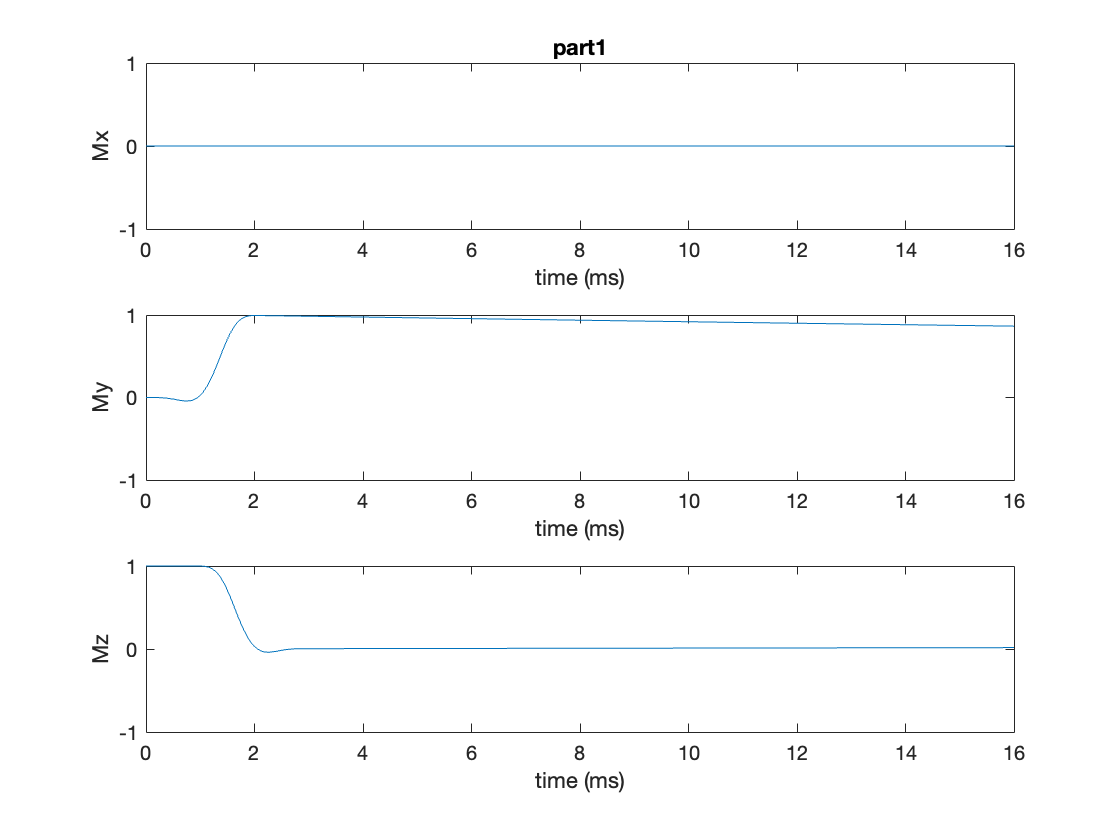
\includegraphics[width=0.8\textwidth]{1.png}
    \caption{ (T1, T2) = (1000,100) ms.}
\end{figure}  
\newpage
%page 2
\section[short]{PART 2}
Applied magnetic field remains the same:
\begin{align*}
B_x &= RF(t) \cos(\omega_{\text{shift}} t) = RF\\
B_y &= RF(t) \sin(\omega_{\text{shift}} t) = 0\\
B_z &= G_{x} x + G_{y} y + G_{z} z = 0
\end{align*}

$M_x$: $M_x$ remains same.\vspace{\baselineskip}

$M_y$: Transverse relaxation $T_2$ is short enough to see the decreasing.\vspace{\baselineskip}

$M_z$: $T_1$ is also short enough to let $M_z$ recover.\vspace{\baselineskip}

$M_y$ component in part 2 shows a decay post-RF pulse, which is not observed in part1, 
due to the shorter $T_2$ relaxation time. For $M_z$, the recovery begins within the time frame shown
 in part2, unlike in part1, where $M_z$ remains at its lower level, due to the much shorter $T_1$
 relaxation time in part 2.

\begin{figure}[hb]
    \centering
    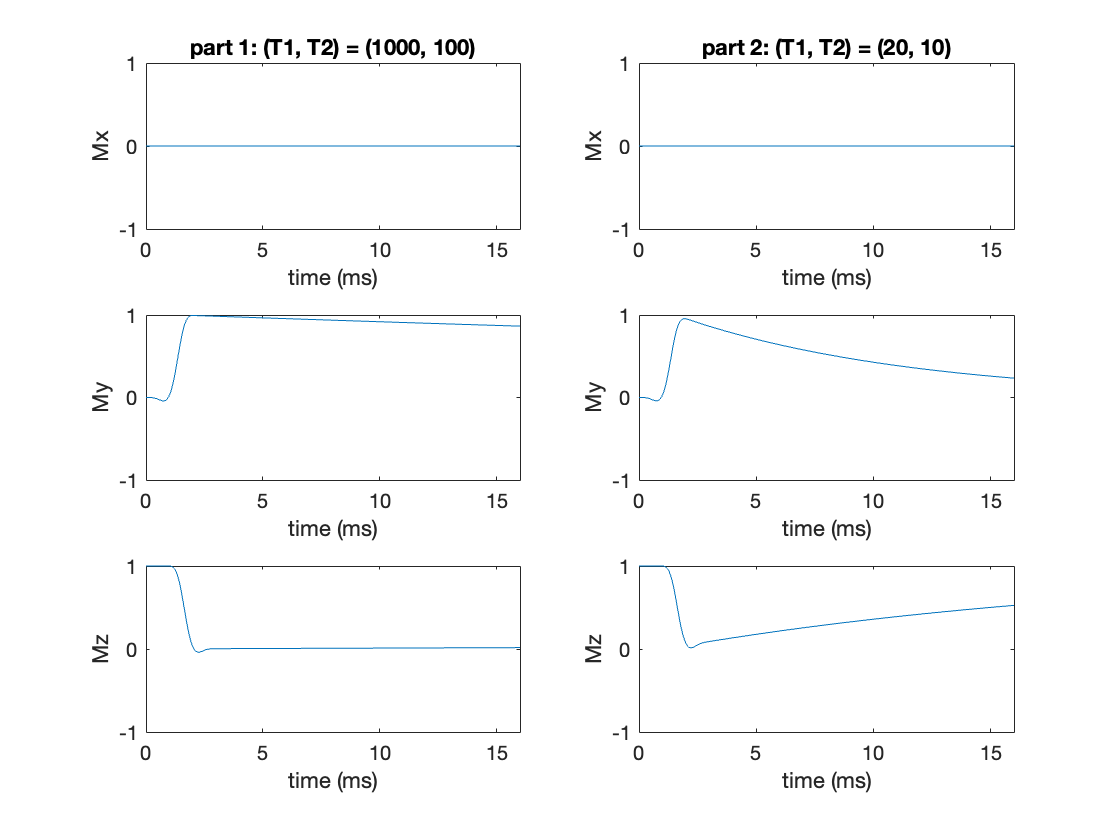
\includegraphics[width=1\textwidth]{2.png}
    \caption{Campare part1 and part2.}
\end{figure}  
\newpage
%page 3
\section[short]{PART 3}
Impliment the followng equation and generate $G_z$ first:
\[
G_z{\text{positive}} = \frac{BW}{\left( \frac{\gamma}{2\pi} \right) \Delta z} = 3.1321 \times 10^{-6}
\]
\[
G_z{\text{negative}} = -G_z{\text{positive}} = -3.1321 \times 10^{-6}
\]

Applied magnetic field remains the same ($z$ remians to be 0, so that $B_z$ remains unchanged):
\begin{align*}
B_x &= RF(t) \cos(\omega_{\text{shift}} t) = RF\\
B_y &= RF(t) \sin(\omega_{\text{shift}} t) = 0\\
B_z &= G_{x} x + G_{y} y + G_{z} z = 0
\end{align*}

$M_x$: $M_x$ remains same as part1.\vspace{\baselineskip}

$M_y$: $M_y$ remains same as part1.\vspace{\baselineskip}

$M_z$: $M_z$ remains same as part1.\vspace{\baselineskip}

Due to the unchanged applied magnetic field, the plot looks exactly same as the plot in part1.

\begin{figure}[hb]
    \centering
    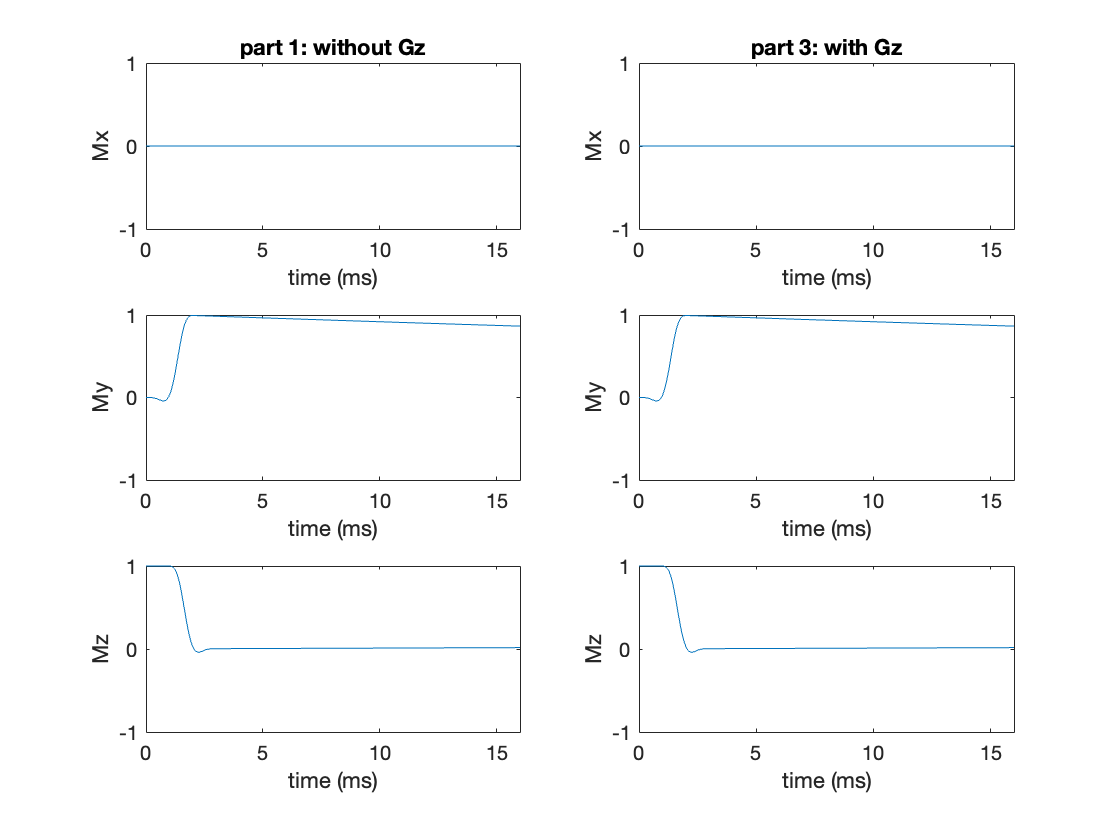
\includegraphics[width=1\textwidth]{3.png}
    \caption{Campare part1 and part3.}
\end{figure}  
\newpage

%page 4
\section[short]{PART 4}
Applied magnetic $B_z$ field was shown significant difference with the changing of $z$
\begin{align*}
    B_z &= G_{x} x + G_{y} y + G_{z} z = G_{z} \times z
\end{align*}

$M_x$: the patterns of $z = 0.2$ and $z = 1.0$ are totally different than $z = 0$\\
$z = 0.2$: initialized with fluctuations, indicating that the gradient has caused some dephasing in the transverse plane.\\
$z = 1.0$: shows significant oscillations after the RF pulse, the dephasing is obviously.\vspace{\baselineskip}

$M_y$:\\ 
$z = 0.2$: there shown a huge fluctuations at the begining, followed with the same pattern as $z = 0$.\\
$z = 1.0$: also shows oscillations but appears to be damping out over time, suggesting the combined effects of 
the RF pulse and the gradient on spins outside the slice.\vspace{\baselineskip}

$M_z$:\\ 
$z = 0.2$: a same pattern as $z = 0$ was shown.\\ $z = 1.0$: increased extremly rapid at the begining, 
followed with a travial recovery, indicating the effect of relaxation was reduced.\vspace{\baselineskip}

\begin{figure}[hb]
    \centering
    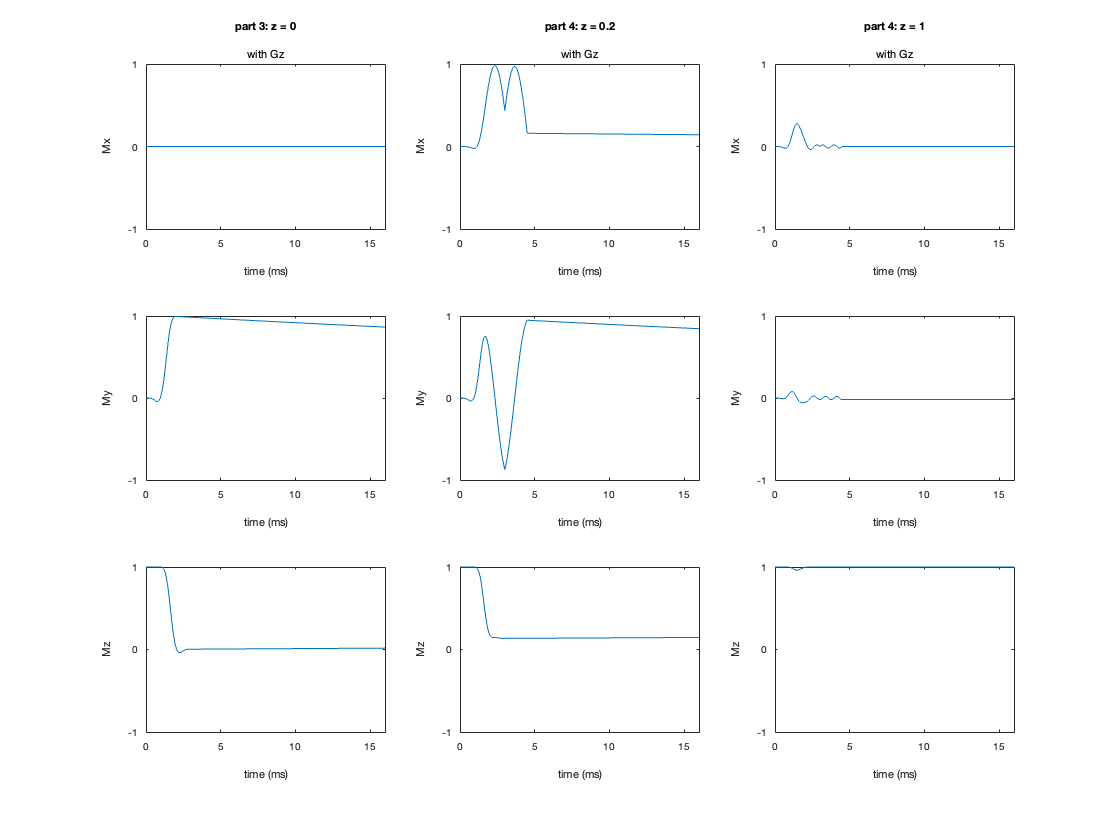
\includegraphics[width=1\textwidth]{4.png}
    \caption{Campared with different $z$.}
\end{figure}
\newpage  
%page 5
\section[short]{PART 5}
The following equation was implimented to generate $G_x{\text{positive}}$ first and $G_x{\text{negative}}$ for symmetrical acquisition:
\[
G_x{\text{positive}} = \frac{N_x \Delta k_x}{\frac{\gamma}{2\pi} T_{\text{read}}} = 1.4682 \times 10^{-5}
\]
\[
G_x{\text{negative}} = \frac{8ms \times -G_x{\text{positive}}}{2 \times 2ms} = - 2.9363 \times 10^{-5}
\]
Applied magnetic $B_z$ field changed because of $G_x$ 
\begin{align*}
    B_z &= G_{x} x + G_{y} y + G_{z} z = G_x \times 4
\end{align*}

$M_x$: $M_x$ remains same bfore the $G_x$ pluse, followed by significant oscillations.\\
$M_y$: $M_y$ remains same bfore the $G_x$ pluse, followed by significant oscillations.\\
$M_z$: $M_z$ remains al most same than part1.\\

The introduction of the x-gradient has introduced dephasing in the transverse plane, which is evident 
from the oscillations in both $M_x$ and $M_y$. This dephasing is a result of the Larmor frequency 
variation across the x-axis due to the x-gradient. The oscillations in $M_x$ and $M_y$ might be indicative of
 a spin echo sequence, where the x-gradient is switched rapidly to refocus the spins' dephasing caused by the z-gradient.
\begin{figure}[hb]
    \centering
    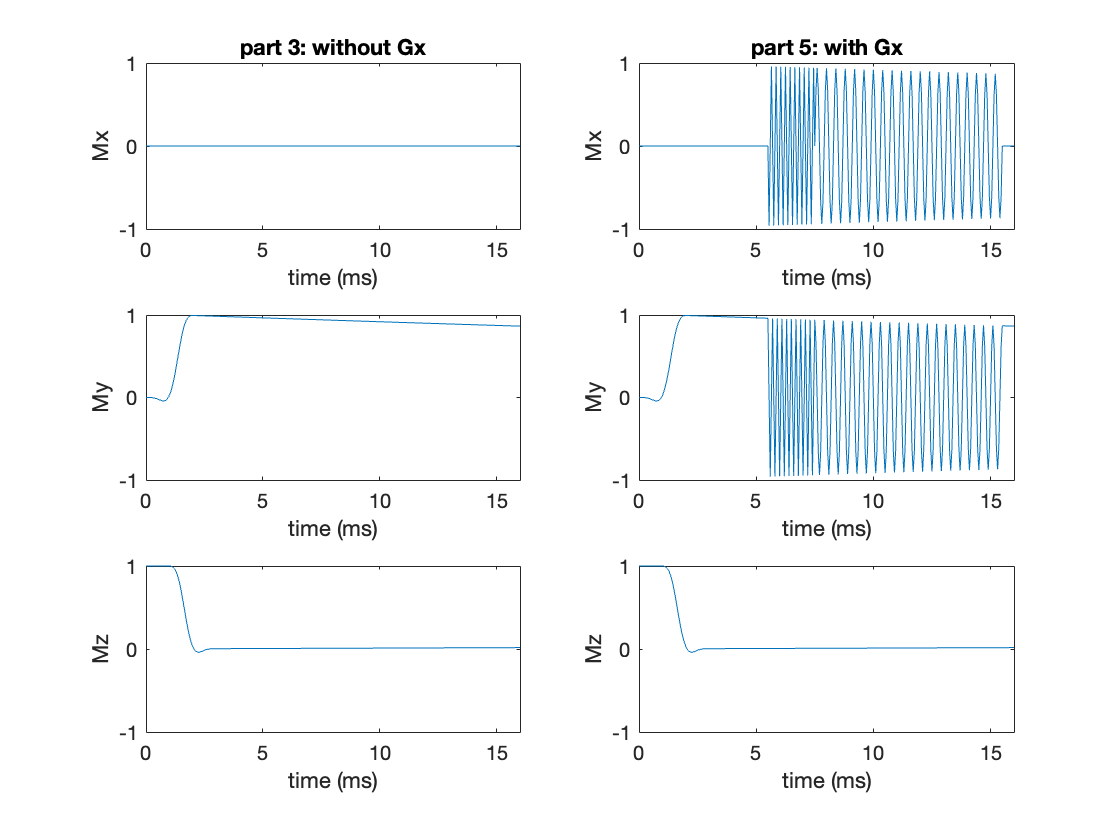
\includegraphics[width=1\textwidth]{5.png}
    \caption{Caption for the figure.}
\end{figure}
\newpage 
%page 6
\section[short]{PART 6}
Axis $x$ was generated to show the variation between signal and $x$:
\begin{align*}
n_{\text{read}} &= 80, \Delta x = \frac{FOV_x}{n_{\text{read}}} = 0.2cm \Rightarrow \\
x &= [-FOV_x/2 + 0 \Delta x, -FOV_x + 2 \Delta x, ... -FOV_x + (n_{\text{read}} - 1) \Delta x, -FOV_x + n_{\text{read}} \Delta x]\\
\end{align*}

From the plot, we can find that the only signal was generated at location $x = 4$. The other
 location remain 0, which correctly describe the step we set up from part1 to part5.\\

 Compared to part3, which did not involve the x gradient, this step in the simulation process 
 includes both the z and x gradients. The presence of the x gradient allows for spatial encoding 
 along the x-axis, which is necessary for image reconstruction.\\

 The main difference is that now the signal can be localized in space due to the spatial encoding 
 provided by the x gradient. In part3, without the x gradient, such spatial localization would not be possible.


\begin{figure}[hb]
    \centering
    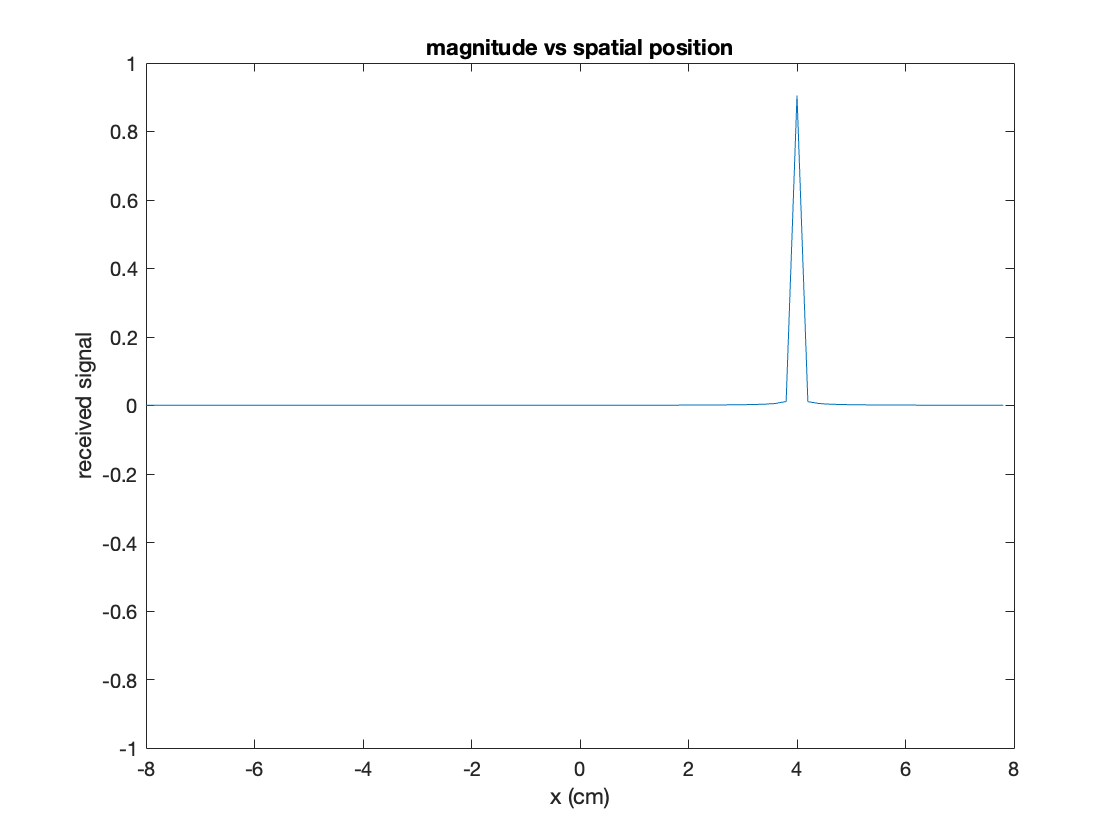
\includegraphics[width=1\textwidth]{6.png}
    \caption{signal vs $x$}
\end{figure}
\newpage 
%page 7
\section[short]{PART 7}
The following equation was implimented to generate $G_y{\text{max}}$ first:
\[
G_y{\text{max}} = \frac{N_y \Delta k_y}{\frac{\gamma}{2\pi} 2 T_y} = 2.9363 \times 10^{-5}
\]
And then phase decoding parameter $\Delta G_y$:
\[
\Delta G_y = \frac{2 \pi}{2 \gamma FOV_y} = 9.7878 \times 10^{-7}
\]
Applied magnetic $B_z$ field changed because of $G_y$ 
\begin{align*}
 B_z &= G_{x} x + G_{y} y + G_{z} z = G_x \times 4 + G_y \times 4 + G_y \times 0
\end{align*}
The $M_{xy}$ was also generated:
\[
 M_{xy} = m_x + i m_y
\]
Finally, axis $k_x$ and $k_y$ were generated to use "image" commend in MATLAB:
\begin{align*}
W_x &= \Delta k_x \times N_X \Rightarrow k_x = [-W_x + 0 \Delta k_x, -W_x + 2 \Delta k_x, ... -W_x + (N_x - 1) \Delta k_x, -W_x + N_x \Delta k_x]\\
W_y &= \Delta k_y \times N_y \Rightarrow k_y = [-W_y + 0 \Delta k_y, -W_y + 2 \Delta k_y, ... -W_y + (N_y - 1) \Delta k_y, -W_y + N_y \Delta k_x]
\end{align*}
From the plot, we can see there was shown uniform stripes in the k-space, indicating 
the single signal was generated inside k-space.
At the same time, the imaginary part was also shown uniform stripes. But they will change significantly in part 10 with $object_{23}$.\\
The real and imaginary parts of the k-space data can be combined to form a complex image, 
which after inverse Fourier transforming, provides both the magnitude and phase images in the spatial domain.
\begin{figure}[hb]
    \centering
    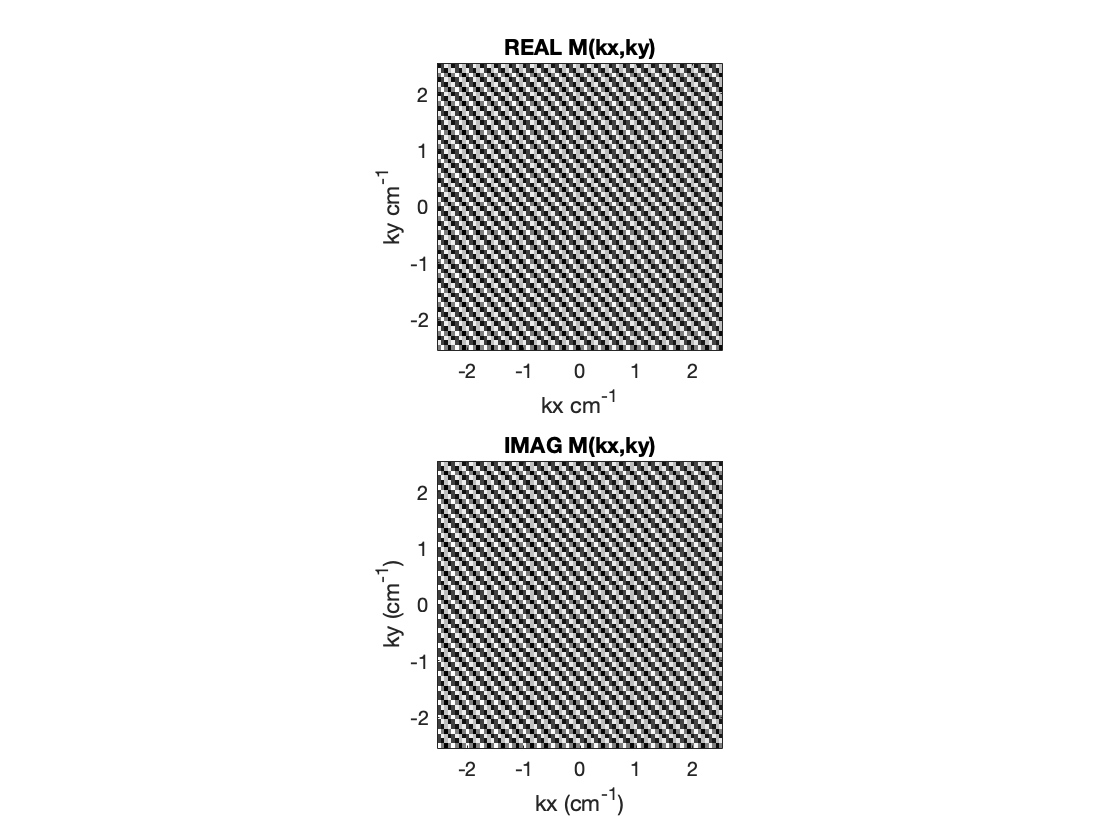
\includegraphics[width=0.75\textwidth]{7.png}
    \caption{Real part and imaginary part.}
\end{figure}
\newpage 
%page 8
\section[short]{PART 8}
The following equation was implimented (2D inverse Fourier transform), and the image was generated:
\[
m(x,y) = F^{-1}_{2D}\{M(k_x(t), k_y(t))\}
\]
Axis $x$ and $y$ were generated to use "image" commend in MATLAB:
\begin{align*}
n_{\text{read}} &= 80, \Delta x = \frac{FOV_x}{n_{\text{read}}} = 0.2cm \Rightarrow \\
x &= [-FOV_x/2 + 0 \Delta x, -FOV_x + 2 \Delta x, ... -FOV_x + (n_{\text{read}} - 1) \Delta x, -FOV_x + n_{\text{read}} \Delta x]\\
n_{\text{pe}} &= \frac{G_y{\text{max}}}{\Delta G_y} = 60, \Delta y = \frac{FOV_y}{n_{\text{pe}}} = 0.2cm \Rightarrow \\
y &= [-FOV_y/2 + 0 \Delta y, -FOV_y + 2 \Delta y, ... -FOV_y + (n_{\text{pe}} - 1) \Delta y, -FOV_y + n_{\text{pe}} \Delta y]
\end{align*}
From the plot, it is obviously that only location $(x,y) = (4,4)$ has pixel image,
 and the value is equal to 1 which is pure white. For the other parts of the image,
 they are all black which means no signal was collected. The single bright spot indicates that the
  simulation has correctly localized the signal from the point object in space. This spot is the 
  result of the MRI sequence encoding spatial information into the phase and frequency of the signal, 
  which is then decoded through the Fourier transform.

\begin{figure}[hb]
    \centering
    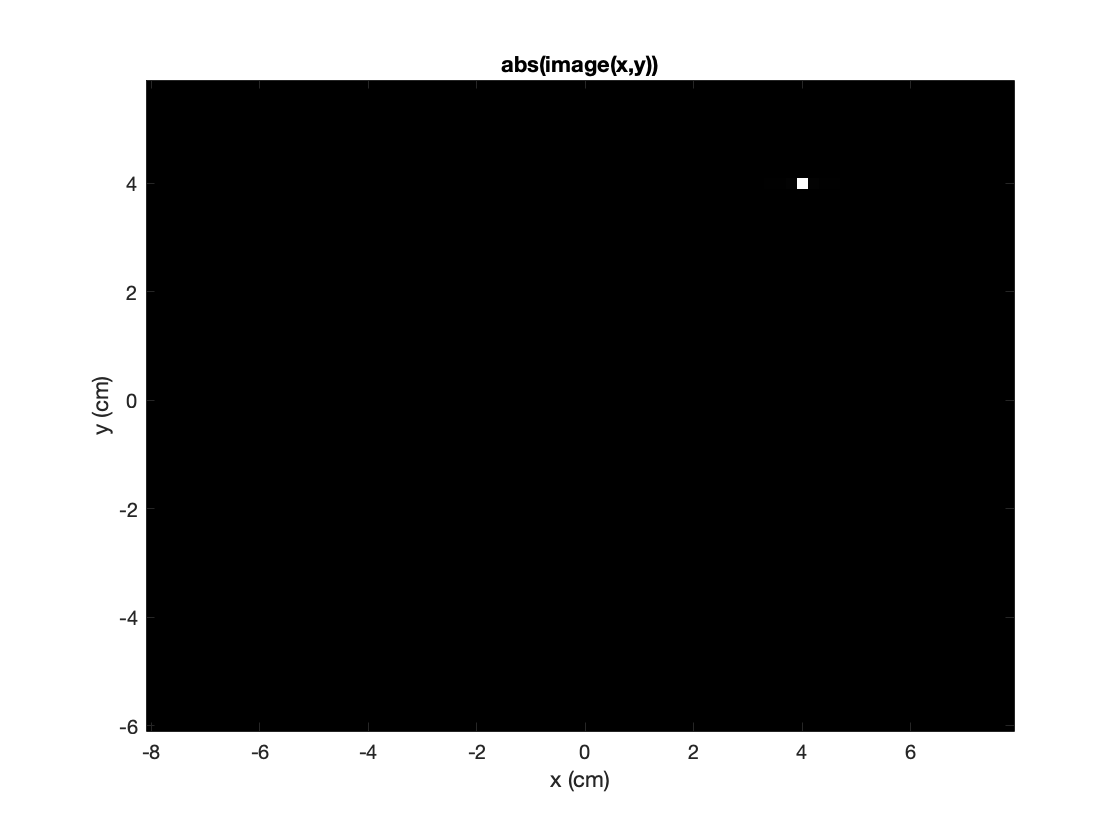
\includegraphics[width=1\textwidth]{8.png}
    \caption{Image after 2D inverse Fourier transform.}
\end{figure}
\newpage 
%page 9
\section[short]{PART 9}
By contrast to the part8, the only thing changed is the position of $y$, which caused the change of 
applied magnetic $B_z$:
\begin{align*}
 B_z &= G_{x} x + G_{y} y + G_{z} z = G_x \times 4 + G_y \times 10 + G_y \times 0
\end{align*}

The FOV is not wide enough to cover the position at +10 cm, but the plot still showed us somthing interesting. 
The spin wrap around to the opposite side of the image due to the aliasing effect, instead of going outside
 the image and disappear. And the location of new pixel of $(x,y)$ is (4,-2).
\begin{figure}[hb]
    \centering
    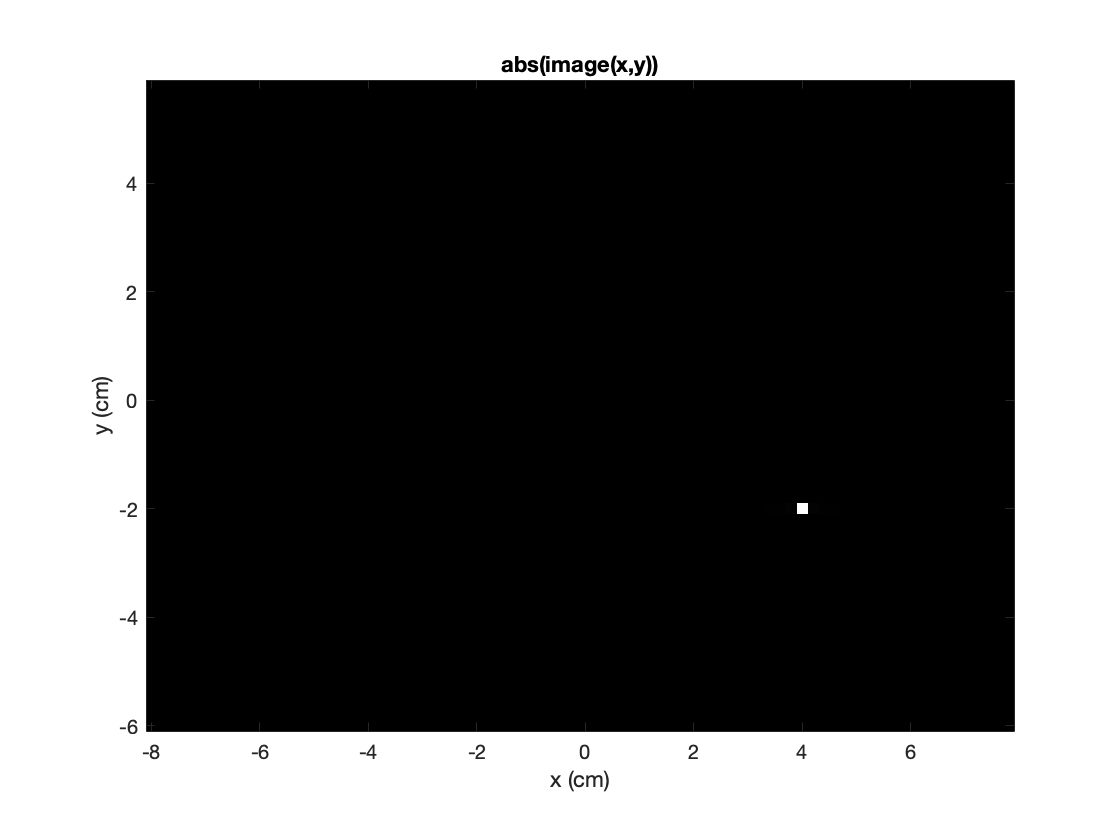
\includegraphics[width=1\textwidth]{9.png}
    \caption{(x,y,z) = (4,10,0).}
\end{figure}
\newpage 
%page 10
\section[short]{PART 10}
The real and imaginary parts of the k-space data typically contain both the amplitude and phase information 
of the signal. The center of the k-space $(k_x=0, k_y=0)$ contains the bulk of the signal power, 
and the surrounding k-space encodes the higher spatial frequencies (details and edges) of the image.\\

The magnitude of the k-space data is a monochrome image showing the distribution of signal intensity across
different spatial frequencies. Bright spots in this image correspond to areas with higher signal power,
which, after inverse Fourier transformation, contribute to the contrast and details in the spatial domain 
image.\\

The object looks like the slice of brain.
\begin{figure}[hb]
    \centering
    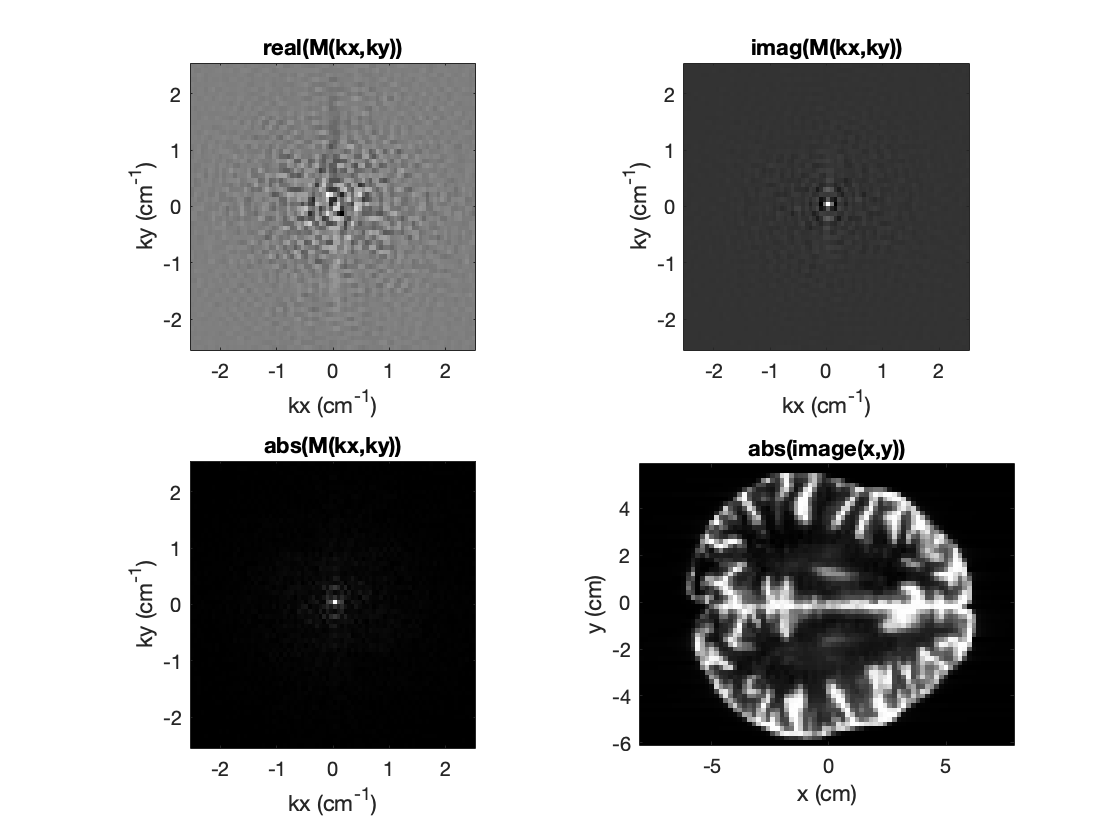
\includegraphics[width=1\textwidth]{11.png}
    \caption{Image for $z_{\text{slice}} = 0$.}
\end{figure}
\newpage 
%page 11
\section[short]{PART 11}
The following equation was implimented, and $z_{\text{slice}} = 1$, which is different than part1 - part10:
\[
    \omega_{\text{shift}} = \gamma G_z z_{\text{slice}} = 8.3776
\]

To simulate the magnetization, the following equation were implimented and changed other than same as part1 - part10:
\begin{align*}
    B_x &= RF(t) \cos(8.3776 t)\\
    B_y &= RF(t) \sin(8.3776 t)\\
    B_z &= G_{x} x + G_{y} y + G_{z} z
\end{align*}
By Impliment same loop in part10, we can generate the following plot, which is different than part10.
By adjusting the slice position and subsequently modifying $B_1$ would result in an image that reflects 
the anatomy or object structure at the new slice location.
\begin{figure}[hb]
    \centering
    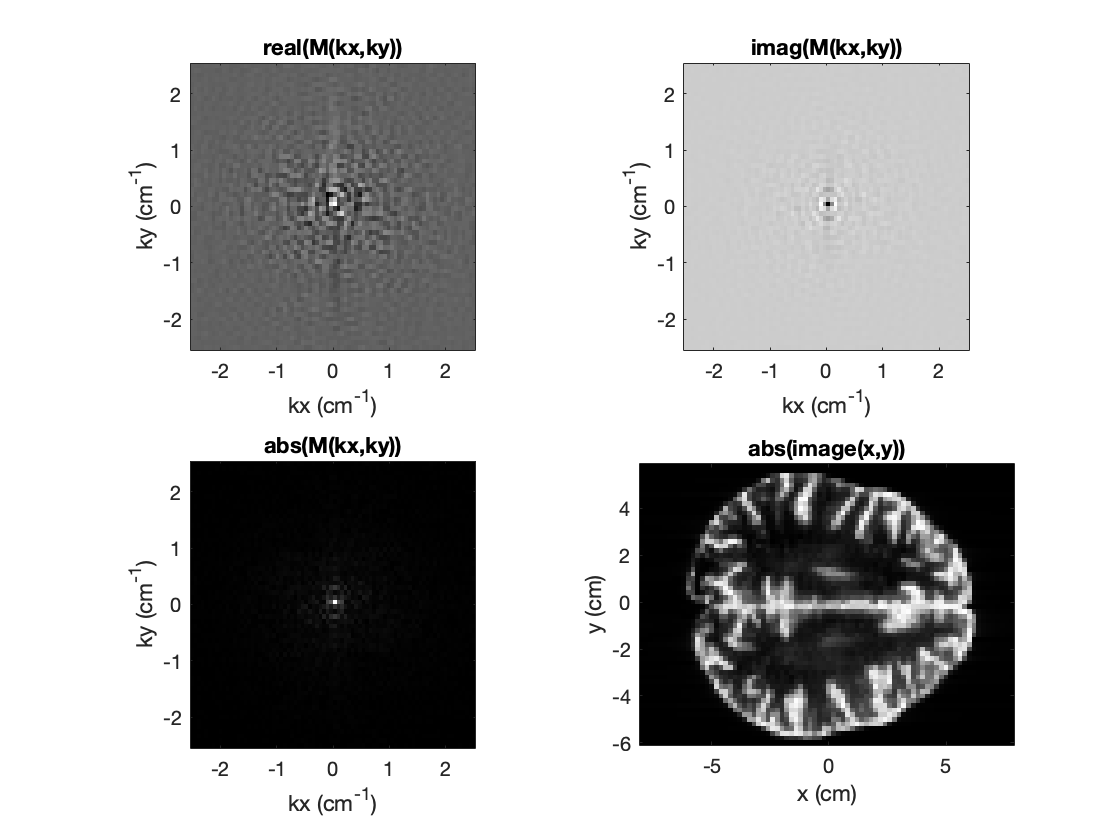
\includegraphics[width=1\textwidth]{12.png}
    \caption{Image for $z_{\text{slice}} = 1$.}
\end{figure}
\newpage 

\end{document}